\chapter{Implementation}\label{ch:implementation}

In this chapter, I am going to analyze my implementation process.
Initially, I will refer to the libraries and the tools that helped me to implement this work.
Next, I will define the DL model.
Finally, I will explain how this model attached to the stream monitoring protocols.

As I said in section~\ref{sec:related-work-and-motivation}, both GM and FGM do not follow the classic parameter server model.
At first glance, the coordinator seems to have this functionality.
Although, the way that decides to make the synchronizations differs from the classic model.
The parameter server synchronizes the workers after some discrete steps while the stream monitoring methods synchronize when a condition is violated.
It leads to a more efficient training process regarding the communication between workers and the coordinator.

At this point, it is essential to note that this work is a simulation of a real system.
The goal of this thesis is to prove that FGM is more efficient than GM in respect of the network cost without losing the accuracy of the ML model.
I achieved this by tracking the communication cost (bytes) between the network workers.


\section{Libraries and Tools}\label{sec:libraries-and-tools}

This project is developed mostly in \emph{C++} and rarely in \emph{Python}.
The library that I handled to track the communication over the workers
is called \emph{ddssim}~\cite{ddssim_repo} and was developed in C++ by my mentor, Vasilis Samoladas.
I used the Python and especially the \emph{Pandas}~\cite{pandas} and \emph{scikit-learn}~\cite{sklearn} libraries to preprocess the NLP data,
and I utilized the \emph{matplotlib}~\cite{matplotlib} library to visualize both data and results.
I used the \emph{mlpack} library~\cite{mlpack2018} for ML purposes, which is written in C++.


\section{Distributed learning using GM protocol}\label{sec:distributed-learning-using-gm-protocol}

I introduced the basic structure of GM protocol in~\ref{subsec:geometric-monitoring}.
I used the Kamp's rebalanced method Kamp to make distributed training.
Both GM and FGM protocols monitor data streams.
For this reason, I should adjust some meanings to the distributed DL concept.
For the distributed training, $S_i(t)$ is the local model parameters (weights) of a site (worker) while $E$ is the average of the local model parameters or the global model.
Besides, the drift vector $X_i(t)$ is the difference between the previous and current model weights.
The threshold $T$ has the same meaning as in the stream monitoring.

\vspace{2cm}

\begin{figure}[H]
    \centering
    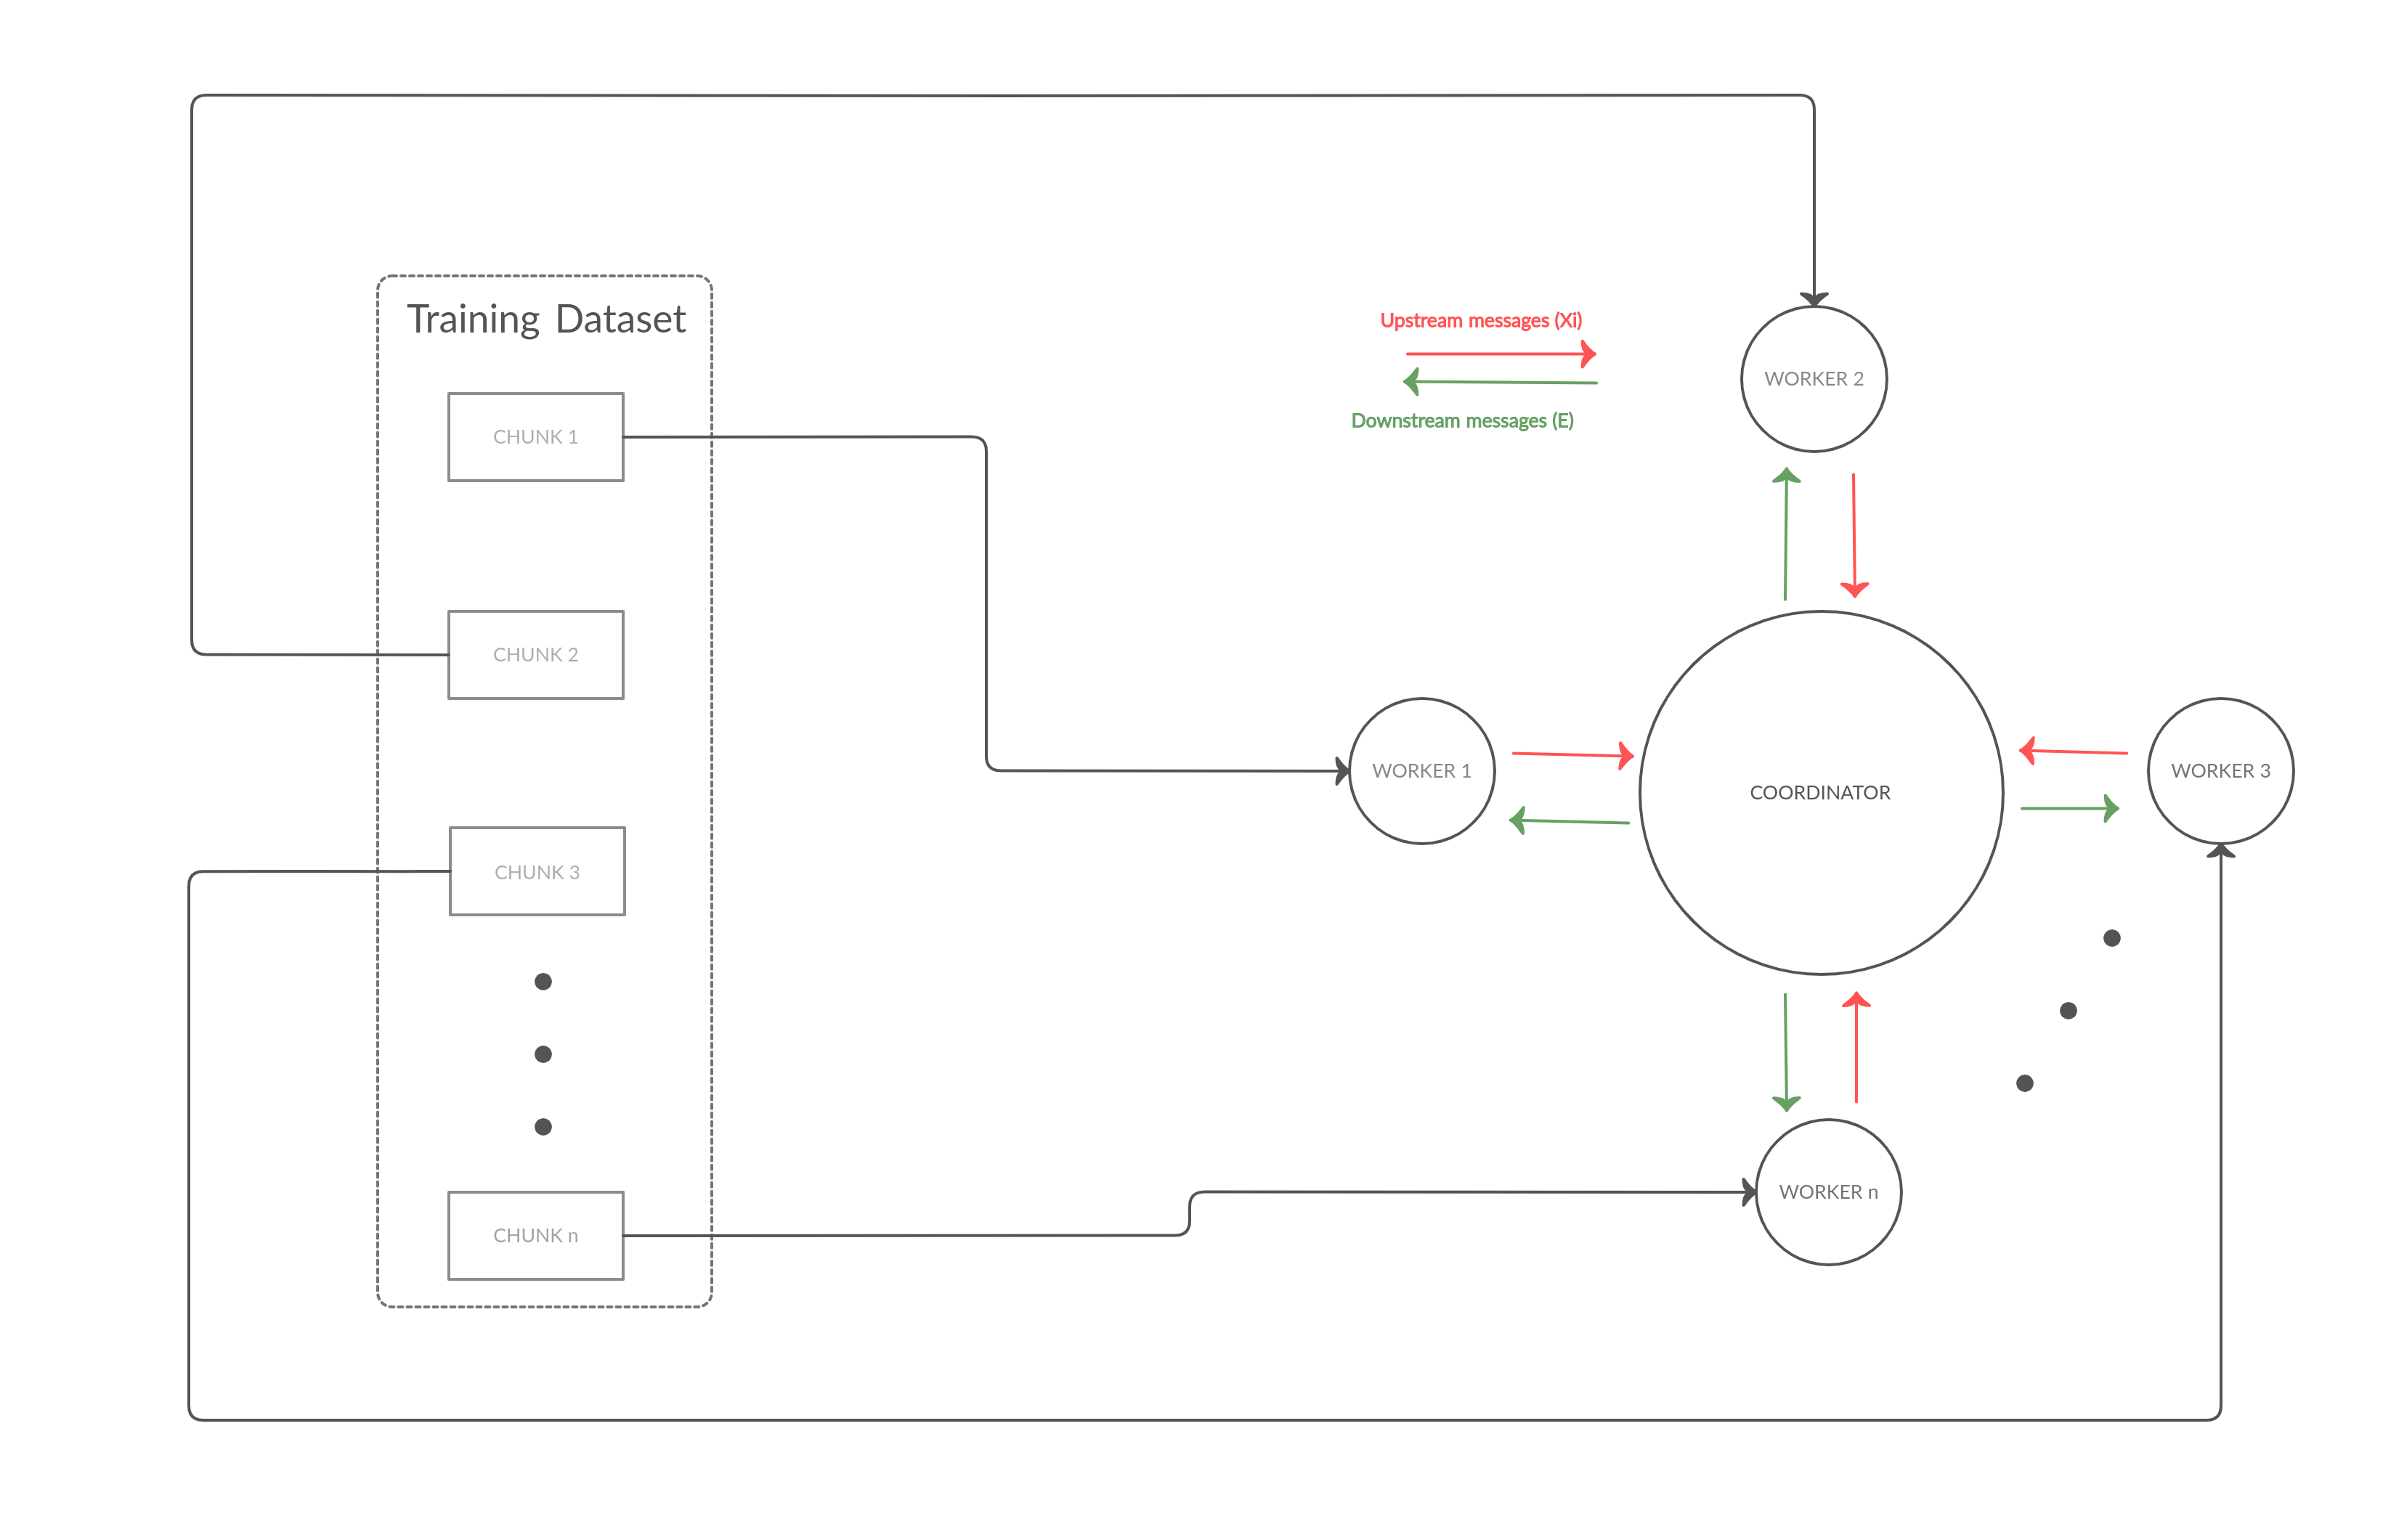
\includegraphics[scale=.125]{./images/impl/arch-gm.png}
    \caption{Coordinator - Worker model for training via GM}
    \label{fig:arch-gm}
\end{figure}

\newpage

The learning process by GM is organized in three (3) phases. \\
In the first phase, the coordinator warms up it's ML model with a small bunch of data.
In this way, the system becomes stable earlier since the other option was to define the global model as a zero vector.
A system is called stable when the pace of new rounds is solid.
After that, the global violation counter $u$ is defined to zero and the global estimate $E$ has as value the warmed up vector.
The global estimate $E$ will be the final trained model.
The first round has already started.

In the second phase, each worker fits a batch of samples to its model.
In other words, at this moment each worker calculates the drift vector which is the difference from the past and the current model parameters vector.
Next, checks if the fresh model violates the local condition (Eq.~\ref{eq:equation33}).
If it is true, this worker sends a violation message to the coordinator.
Else, it keeps going by fitting the next batch of samples.

The third and the last phase concerns the coordinator.
In this phase, the coordinator should handle the situation that resulted from the previous phase.
Initially, the hub checks if the workers that have violated the condition are equal to the total number of the system workers.
If it's true, then the hub sets a new global estimate averaging all the workers' model parameters.
Then it sends the new model to all workers.
Otherwise, it aggregates and sends only the model parameters from the workers who have violated the local condition.

\vspace{1cm}

Following, I present the algorithm that describes the process of distributed training using the GM protocol which is based on~\ref{subsec:geometric-monitoring}


\begin{algorithm}[H]
    \caption{Learning process via GM}
    \begin{algorithmic}[1]

        \vspace{0.05in}
        \REQUIRE T (threshold), k (\# workers)
        \vspace{0.05in}

        \phase{Initialization}
        \vspace{-2.5ex}
        \STATE \textbf{warm up} the global learner (coordinator) and \textbf{take} the initial weights $w_0$
        \STATE \emph{violation counter} $v \leftarrow 0$
        \STATE \emph{global estimate} $E \leftarrow w_{init}$

        \phase{Round $n$ at worker $i$}
        \vspace{-2.5ex}
        \STATE \textbf{fit} a batch of samples to the local model and calculate the new drift vector $X_i$
        \IF{$||X_i(n) - E ||^2_2 > T$}
        \STATE \textbf{send} $w_{n,i}$ to coordinator \COMMENT{\textbf{violation}}
        \ENDIF

        \phase{The coordinator deals with a local violation}
        \vspace{-2.5ex}
        \STATE \textbf{let} $B$ the set of workers that have violated the condition
        \STATE $v \leftarrow v + |B|$
        \IF{$u = k$}
        \STATE $B \leftarrow [ \,k] \,$
        \ENDIF
        \WHILE{$B \neq [ \,k] \,$ \textbf{and} $\frac{1}{k} \sum_{j\in B}^{} ||X_j(n) - E ||^2_2 > T$}
        \STATE \textbf{receive} model parameters from workers $\in B$
        \ENDWHILE
        \STATE \textbf{send} model parameters $S(n) = \frac{1}{|B|} \sum_{j\in B}^{} X_j(n)$ to workers $\in B$
        \IF{$B = [ \,k] \,$}
        \STATE \textbf{set} a new global estimate $E \leftarrow S(n)$
        \ENDIF

    \end{algorithmic}\label{alg:rnn_gm}
\end{algorithm}


\section{Distributed learning using FGM protocol}\label{sec:distributed-learning-using-fgm-protocol}

To describe the learning process using the FGM protocol, I based on the basic structure that I have quoted in~\ref{subsec:functional-geometric-monitoring}.

{\large \textbf{Safe function}}

The GM protocol handles the safe zone condition of Eq~\ref{eq:equation33} to synchronize the learners.
This time, I adopted and adjusted~\cite{samoladas_functional_nodate} this safe zone to a real safe zone function $\phi : V \rightarrow R$, to match with FGM protocol.
The admissible region $A$ is the convex level set

\begin{equation}
    A = \{ x | \norm{x}_2 \geq (1 - T) \norm{E}\}\label{eq:equation35}
\end{equation}


Next, the safe function can be combined via the point-wise max operation:

\begin{equation}
    \phi(X,E) = max\{-T\norm{E} - X\frac{E}{\norm{E}}, \norm{X+E} - (1+T)\norm{E}\}\label{eq:equation36}
\end{equation}

where $X$ is the drift vector of a worker.

{\large \textbf{Learning by FGM}}

In the beginning of~\ref{sec:distributed-learning-using-gm-protocol} I mentioned to the variables that both algorithms have.
Not only GM but also FGM has the same meanings to these variables (e.g $E, X_i, T$).
The FGM has an additional variable, the $\epsilon_\psi$ which is a small number that is not related to the desired accuracy query $\epsilon$ (or $T$),
but only to the desired quantization for monitoring $\psi$.

\vspace{2cm}

\begin{figure}[H]
    \centering
    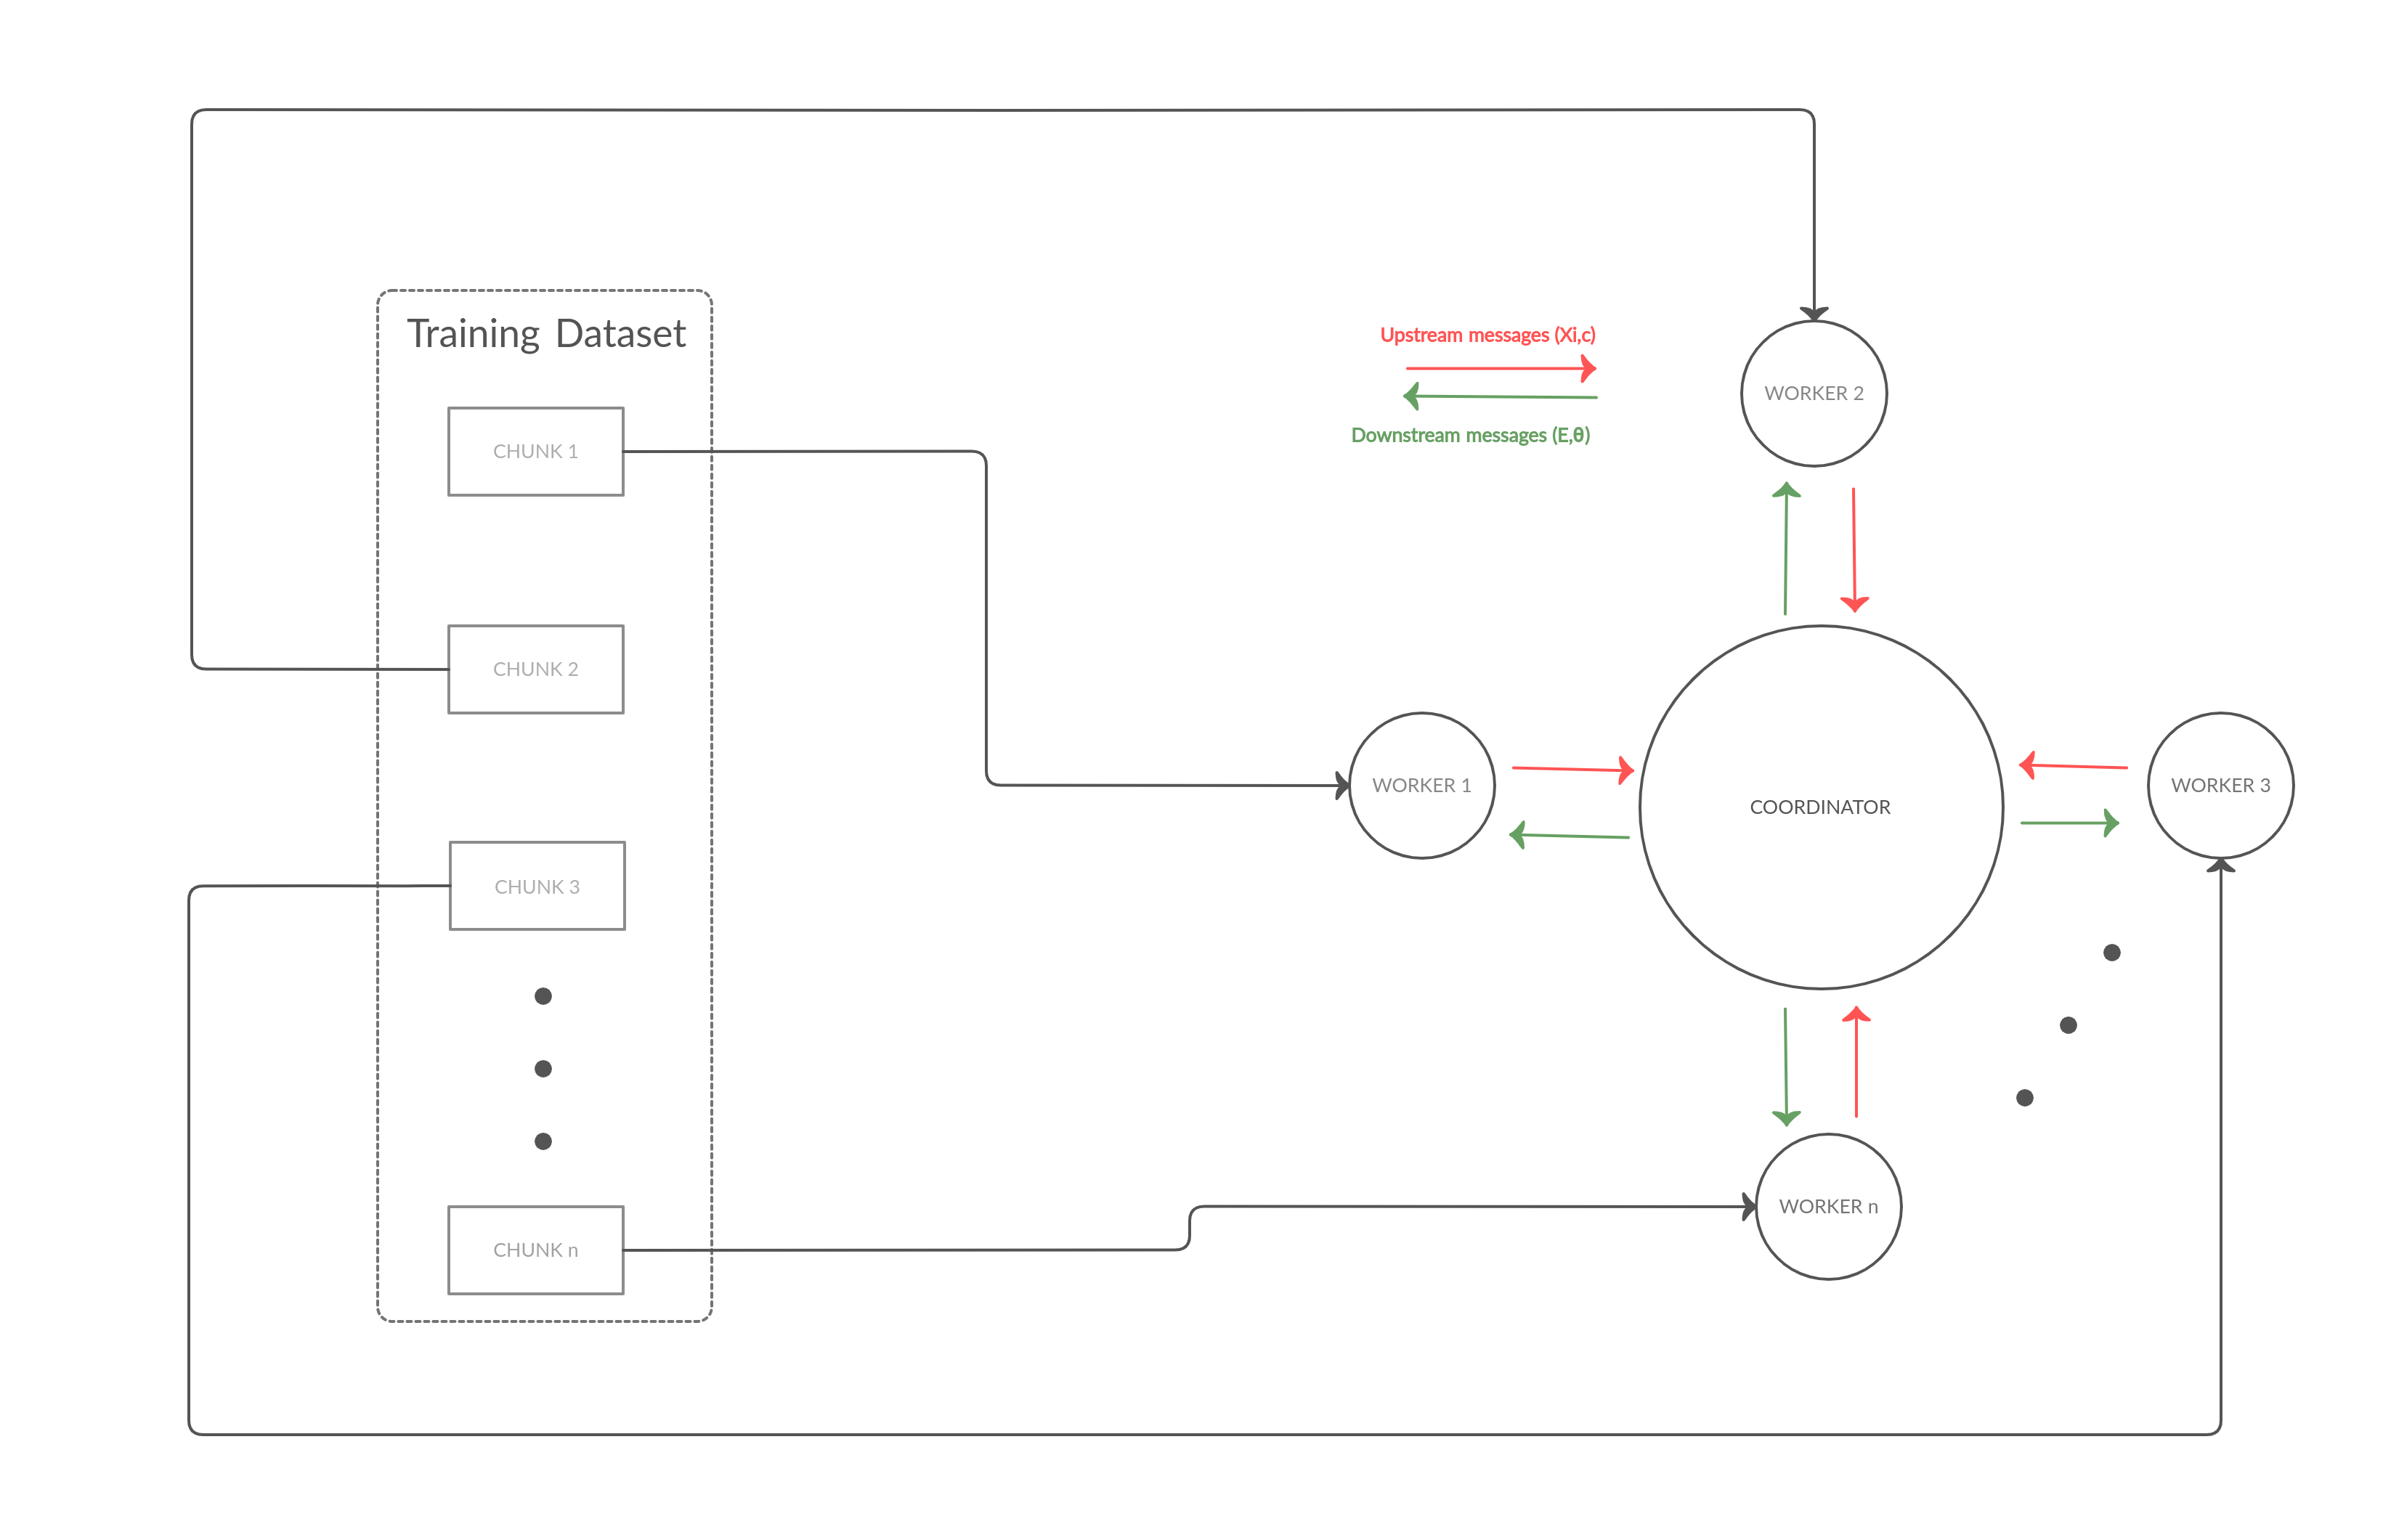
\includegraphics[scale=.125]{./images/impl/arch-fgm.png}
    \caption{Coordinator - Worker model for training via FGM}
    \label{fig:arch-fgm}
\end{figure}

\newpage

The learning process by FGM is organized in four (4) phases. \\
In the first phase, as in GM, the coordinator warms up it's ML model with a small bunch of data.
After that, the global counter $c$ is defined to zero and the global estimate $E$ has as value the warmed up vector.
Additionally, $\psi$ and quantum $\theta$ takes the initial value as it defined in subsection~\ref{subsec:functional-geometric-monitoring}. \\
The first round has already started.

In the second phase, the worker has received the global estimate $E$ and the quantum $\theta$ and updates its corresponding variable.
The difference between the second and third phases is the update of $E$, which is not needed for the start of a new sub-round in phase 3.


In the fourth phase, each worker fits a batch of samples to its model as the third one in GM.
Next, checks if violates the local condition (Eq.~\ref{eq:equation34b}).
If it is true, this worker sends the local increment to the coordinator.
Else, it keeps going by fitting the next batch of samples.

In the fifth phase, the coordinator should check if the increment that has received leads to a violation.
Initially, the hub sums the received increment to the global counter.
If the global counter is greater than the total number of the system workers, then the hub calculates the $\psi$.
If $\psi$ is greater or equal to $\epsilon_\psi k \phi(\overrightarrow{\rm 0})$ then the coordinator sets the variables and routes a new round.
Otherwise, a new sub-round starts.

\vspace{1cm}

Below, I present the algorithm that describes the process of distributed training using the FGM protocol.


\begin{algorithm}[h!]
    \caption{Learning process via FGM}
    \begin{algorithmic}[1]

        \vspace{0.05in}
        \REQUIRE $\phi$ (safe function), $\epsilon_\psi$, k (\# workers)
        \vspace{0.05in}

        \phase{Initialization}
        \vspace{-2.5ex}
        \STATE \textbf{warm up} the global learner (coordinator) and \textbf{take} the initial weights $w_0$
        \STATE \emph{global estimate} $E \leftarrow w_0$
        \STATE \emph{global counter} $c \leftarrow 0$
        \STATE $\psi \leftarrow k \phi(\overrightarrow{\rm 0}, E)$
        \STATE \emph{quantum} $\theta \leftarrow -\frac{\psi}{2k}$

        \phase{Starting a new round: Worker $i$ receives $E$ and $\theta$}
        \vspace{-2.5ex}
        \STATE \textbf{update} the drift vector $X_i \leftarrow E$
        \STATE $quantum \leftarrow \theta$
        \STATE \emph{local counter} $c_i \leftarrow 0$
        \STATE $z_i \leftarrow \phi(X_i, E)$

        \phase{Starting a new subround: Worker $i$ receives $\theta$}
        \vspace{-2.5ex}
        \STATE $c_i \leftarrow 0$
        \STATE $quantum \leftarrow \theta$
        \STATE $z_i \leftarrow \phi(X_i, E)$

        \phase{Worker $i$ fits a batch of samples}
        \vspace{-2.5ex}
        \STATE \textbf{fit} a batch of samples to the local model and calculate the new drift vector $X_i$
        \STATE $quantum \leftarrow \theta$
        \STATE $z_i \leftarrow \phi(X_i, E)$
        \STATE $currentC_i = \lfloor \frac{\phi(X_i,E) - z_i}{\theta} \rfloor$
        \STATE $maxC_i = \max(currentC_i, c_i)$
        \IF{$maxC_i \neq c_i$}
        \STATE $incr_i = maxC_i - c_i$
        \STATE $c_i = currentC_i$
        \STATE \textbf{send} increment $incr_i$ to the coordinator
        \ENDIF

        \phase{Coordinator receives an increment $incr_i$}
        \vspace{-2.5ex}
        \STATE $c \leftarrow c + incr_i$
        \IF{$c > k$}
        \STATE \textbf{collect} all $\phi(X_i,E)$ from all workers
        \STATE $\psi \leftarrow \sum_{1}^{k} \phi(X_i, E)$
        \IF{$\psi \geq \epsilon_\psi k \phi(\overrightarrow{\rm 0})$}
        \STATE \textbf{send} $E$ and $\theta$ to all workers and \textbf{goto} \emph{Phase 2} \COMMENT{\textbf{round condition violation}}
        \ELSE
        \STATE $c \leftarrow 0$
        \STATE $\theta \leftarrow -\frac{\psi}{2k}$
        \STATE \textbf{send} $\theta$ to all workers and \textbf{goto} \emph{Phase 3} \COMMENT{\textbf{subround condition violation}}
        \ENDIF
        \ENDIF

    \end{algorithmic}\label{alg:rnn_fgm}
\end{algorithm}
